% Options for packages loaded elsewhere
\PassOptionsToPackage{unicode}{hyperref}
\PassOptionsToPackage{hyphens}{url}
%
\documentclass[
  11pt,
]{article}
\usepackage{amsmath,amssymb}
\usepackage[]{mathpazo}
\usepackage{ifxetex,ifluatex}
\ifnum 0\ifxetex 1\fi\ifluatex 1\fi=0 % if pdftex
  \usepackage[T1]{fontenc}
  \usepackage[utf8]{inputenc}
  \usepackage{textcomp} % provide euro and other symbols
\else % if luatex or xetex
  \usepackage{unicode-math}
  \defaultfontfeatures{Scale=MatchLowercase}
  \defaultfontfeatures[\rmfamily]{Ligatures=TeX,Scale=1}
\fi
% Use upquote if available, for straight quotes in verbatim environments
\IfFileExists{upquote.sty}{\usepackage{upquote}}{}
\IfFileExists{microtype.sty}{% use microtype if available
  \usepackage[]{microtype}
  \UseMicrotypeSet[protrusion]{basicmath} % disable protrusion for tt fonts
}{}
\makeatletter
\@ifundefined{KOMAClassName}{% if non-KOMA class
  \IfFileExists{parskip.sty}{%
    \usepackage{parskip}
  }{% else
    \setlength{\parindent}{0pt}
    \setlength{\parskip}{6pt plus 2pt minus 1pt}}
}{% if KOMA class
  \KOMAoptions{parskip=half}}
\makeatother
\usepackage{xcolor}
\IfFileExists{xurl.sty}{\usepackage{xurl}}{} % add URL line breaks if available
\IfFileExists{bookmark.sty}{\usepackage{bookmark}}{\usepackage{hyperref}}
\hypersetup{
  pdftitle={Tesis de licenciatura en Biología de Dahiana GuzmánDiseño, análisis.},
  hidelinks,
  pdfcreator={LaTeX via pandoc}}
\urlstyle{same} % disable monospaced font for URLs
\usepackage[margin=1in]{geometry}
\usepackage{color}
\usepackage{fancyvrb}
\newcommand{\VerbBar}{|}
\newcommand{\VERB}{\Verb[commandchars=\\\{\}]}
\DefineVerbatimEnvironment{Highlighting}{Verbatim}{commandchars=\\\{\}}
% Add ',fontsize=\small' for more characters per line
\usepackage{framed}
\definecolor{shadecolor}{RGB}{248,248,248}
\newenvironment{Shaded}{\begin{snugshade}}{\end{snugshade}}
\newcommand{\AlertTok}[1]{\textcolor[rgb]{0.94,0.16,0.16}{#1}}
\newcommand{\AnnotationTok}[1]{\textcolor[rgb]{0.56,0.35,0.01}{\textbf{\textit{#1}}}}
\newcommand{\AttributeTok}[1]{\textcolor[rgb]{0.77,0.63,0.00}{#1}}
\newcommand{\BaseNTok}[1]{\textcolor[rgb]{0.00,0.00,0.81}{#1}}
\newcommand{\BuiltInTok}[1]{#1}
\newcommand{\CharTok}[1]{\textcolor[rgb]{0.31,0.60,0.02}{#1}}
\newcommand{\CommentTok}[1]{\textcolor[rgb]{0.56,0.35,0.01}{\textit{#1}}}
\newcommand{\CommentVarTok}[1]{\textcolor[rgb]{0.56,0.35,0.01}{\textbf{\textit{#1}}}}
\newcommand{\ConstantTok}[1]{\textcolor[rgb]{0.00,0.00,0.00}{#1}}
\newcommand{\ControlFlowTok}[1]{\textcolor[rgb]{0.13,0.29,0.53}{\textbf{#1}}}
\newcommand{\DataTypeTok}[1]{\textcolor[rgb]{0.13,0.29,0.53}{#1}}
\newcommand{\DecValTok}[1]{\textcolor[rgb]{0.00,0.00,0.81}{#1}}
\newcommand{\DocumentationTok}[1]{\textcolor[rgb]{0.56,0.35,0.01}{\textbf{\textit{#1}}}}
\newcommand{\ErrorTok}[1]{\textcolor[rgb]{0.64,0.00,0.00}{\textbf{#1}}}
\newcommand{\ExtensionTok}[1]{#1}
\newcommand{\FloatTok}[1]{\textcolor[rgb]{0.00,0.00,0.81}{#1}}
\newcommand{\FunctionTok}[1]{\textcolor[rgb]{0.00,0.00,0.00}{#1}}
\newcommand{\ImportTok}[1]{#1}
\newcommand{\InformationTok}[1]{\textcolor[rgb]{0.56,0.35,0.01}{\textbf{\textit{#1}}}}
\newcommand{\KeywordTok}[1]{\textcolor[rgb]{0.13,0.29,0.53}{\textbf{#1}}}
\newcommand{\NormalTok}[1]{#1}
\newcommand{\OperatorTok}[1]{\textcolor[rgb]{0.81,0.36,0.00}{\textbf{#1}}}
\newcommand{\OtherTok}[1]{\textcolor[rgb]{0.56,0.35,0.01}{#1}}
\newcommand{\PreprocessorTok}[1]{\textcolor[rgb]{0.56,0.35,0.01}{\textit{#1}}}
\newcommand{\RegionMarkerTok}[1]{#1}
\newcommand{\SpecialCharTok}[1]{\textcolor[rgb]{0.00,0.00,0.00}{#1}}
\newcommand{\SpecialStringTok}[1]{\textcolor[rgb]{0.31,0.60,0.02}{#1}}
\newcommand{\StringTok}[1]{\textcolor[rgb]{0.31,0.60,0.02}{#1}}
\newcommand{\VariableTok}[1]{\textcolor[rgb]{0.00,0.00,0.00}{#1}}
\newcommand{\VerbatimStringTok}[1]{\textcolor[rgb]{0.31,0.60,0.02}{#1}}
\newcommand{\WarningTok}[1]{\textcolor[rgb]{0.56,0.35,0.01}{\textbf{\textit{#1}}}}
\usepackage{graphicx}
\makeatletter
\def\maxwidth{\ifdim\Gin@nat@width>\linewidth\linewidth\else\Gin@nat@width\fi}
\def\maxheight{\ifdim\Gin@nat@height>\textheight\textheight\else\Gin@nat@height\fi}
\makeatother
% Scale images if necessary, so that they will not overflow the page
% margins by default, and it is still possible to overwrite the defaults
% using explicit options in \includegraphics[width, height, ...]{}
\setkeys{Gin}{width=\maxwidth,height=\maxheight,keepaspectratio}
% Set default figure placement to htbp
\makeatletter
\def\fps@figure{htbp}
\makeatother
\setlength{\emergencystretch}{3em} % prevent overfull lines
\providecommand{\tightlist}{%
  \setlength{\itemsep}{0pt}\setlength{\parskip}{0pt}}
\setcounter{secnumdepth}{5}
\usepackage{pdflscape} \newcommand{\blandscape}{\begin{landscape}} \newcommand{\elandscape}{\end{landscape}} \usepackage{float} \floatplacement{figure}{H} \newcommand{\beginsupplement}{ \setcounter{table}{0} \renewcommand{\thetable}{S\arabic{table}} \setcounter{figure}{0} \renewcommand{\thefigure}{S\arabic{figure}} }
\ifluatex
  \usepackage{selnolig}  % disable illegal ligatures
\fi
\newlength{\cslhangindent}
\setlength{\cslhangindent}{1.5em}
\newlength{\csllabelwidth}
\setlength{\csllabelwidth}{3em}
\newenvironment{CSLReferences}[2] % #1 hanging-ident, #2 entry spacing
 {% don't indent paragraphs
  \setlength{\parindent}{0pt}
  % turn on hanging indent if param 1 is 1
  \ifodd #1 \everypar{\setlength{\hangindent}{\cslhangindent}}\ignorespaces\fi
  % set entry spacing
  \ifnum #2 > 0
  \setlength{\parskip}{#2\baselineskip}
  \fi
 }%
 {}
\usepackage{calc}
\newcommand{\CSLBlock}[1]{#1\hfill\break}
\newcommand{\CSLLeftMargin}[1]{\parbox[t]{\csllabelwidth}{#1}}
\newcommand{\CSLRightInline}[1]{\parbox[t]{\linewidth - \csllabelwidth}{#1}\break}
\newcommand{\CSLIndent}[1]{\hspace{\cslhangindent}#1}

\title{Tesis de licenciatura en Biología de Dahiana GuzmánDiseño,
análisis.}
\author{true}
\date{julio 17, 2022}

\begin{document}
\maketitle

\hypertarget{diseuxf1o-de-malla}{%
\section{Diseño de malla}\label{diseuxf1o-de-malla}}

Basado en: Batlle (2021)

\begin{Shaded}
\begin{Highlighting}[]
\CommentTok{\# Crear cuadrícula para diseño de muestreo}
\FunctionTok{library}\NormalTok{(dplyr)}
\end{Highlighting}
\end{Shaded}

\begin{verbatim}
## Warning: replacing previous import 'lifecycle::last_warnings' by
## 'rlang::last_warnings' when loading 'pillar'
\end{verbatim}

\begin{verbatim}
## 
## Attaching package: 'dplyr'
\end{verbatim}

\begin{verbatim}
## The following objects are masked from 'package:stats':
## 
##     filter, lag
\end{verbatim}

\begin{verbatim}
## The following objects are masked from 'package:base':
## 
##     intersect, setdiff, setequal, union
\end{verbatim}

\begin{Shaded}
\begin{Highlighting}[]
\FunctionTok{library}\NormalTok{(sf)}
\end{Highlighting}
\end{Shaded}

\begin{verbatim}
## Linking to GEOS 3.10.1, GDAL 3.4.0, PROJ 8.2.0; sf_use_s2() is TRUE
\end{verbatim}

\begin{Shaded}
\begin{Highlighting}[]
\NormalTok{construir\_cuadricula }\OtherTok{\textless{}{-}}\NormalTok{ T}
\end{Highlighting}
\end{Shaded}

\begin{Shaded}
\begin{Highlighting}[]
\NormalTok{parque }\OtherTok{\textless{}{-}} \FunctionTok{st\_read}\NormalTok{(}\StringTok{\textquotesingle{}data/limite{-}parque.gpkg\textquotesingle{}}\NormalTok{) }\CommentTok{\# Creada en QGIS, ver nota abajo}
\end{Highlighting}
\end{Shaded}

\begin{verbatim}
## Reading layer `limite-parque' from data source 
##   `/home/jose/Documentos/tesis-dahiana/tesis-licenciatura-biologia-uasd-/data/limite-parque.gpkg' 
##   using driver `GPKG'
## Simple feature collection with 1 feature and 1 field
## Geometry type: POLYGON
## Dimension:     XY
## Bounding box:  xmin: 402699.2 ymin: 2041878 xmax: 403116 ymax: 2042246
## Projected CRS: WGS 84 / UTM zone 19N
\end{verbatim}

\begin{Shaded}
\begin{Highlighting}[]
\NormalTok{cuad }\OtherTok{\textless{}{-}} \FunctionTok{st\_read}\NormalTok{(}\StringTok{\textquotesingle{}data/cuadricula.gpkg\textquotesingle{}}\NormalTok{)}
\end{Highlighting}
\end{Shaded}

\begin{verbatim}
## Reading layer `cuadricula' from data source 
##   `/home/jose/Documentos/tesis-dahiana/tesis-licenciatura-biologia-uasd-/data/cuadricula.gpkg' 
##   using driver `GPKG'
## Simple feature collection with 63 features and 5 fields
## Geometry type: POLYGON
## Dimension:     XY
## Bounding box:  xmin: 402637.3 ymin: 2041765 xmax: 403203.5 ymax: 2042297
## Projected CRS: WGS 84 / UTM zone 19N
\end{verbatim}

\begin{Shaded}
\begin{Highlighting}[]
\FunctionTok{plot}\NormalTok{(parque }\SpecialCharTok{\%\textgreater{}\%}\NormalTok{ st\_geometry)}
\FunctionTok{plot}\NormalTok{(cuad }\SpecialCharTok{\%\textgreater{}\%}\NormalTok{ st\_geometry, }\AttributeTok{add=}\NormalTok{T)}
\end{Highlighting}
\end{Shaded}

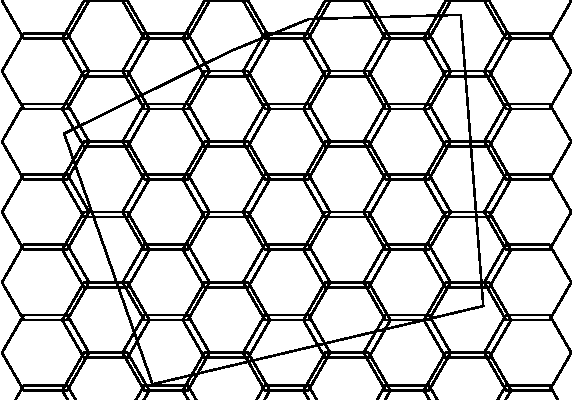
\includegraphics{README_files/figure-latex/unnamed-chunk-3-1.pdf}

\begin{Shaded}
\begin{Highlighting}[]
\NormalTok{cuad2 }\OtherTok{\textless{}{-}} \FunctionTok{st\_as\_sf}\NormalTok{(cuad)}
\NormalTok{cuad2 }\OtherTok{\textless{}{-}}\NormalTok{ cuad2 }\SpecialCharTok{\%\textgreater{}\%}
  \FunctionTok{mutate}\NormalTok{(}
    \AttributeTok{ENLACE=}\DecValTok{1}\SpecialCharTok{:}\FunctionTok{nrow}\NormalTok{(cuad2),}
    \AttributeTok{AREASQM1=}\FunctionTok{st\_area}\NormalTok{(geom) }\SpecialCharTok{\%\textgreater{}\%}\NormalTok{ units}\SpecialCharTok{::}\FunctionTok{drop\_units}\NormalTok{())}
\NormalTok{cuad3 }\OtherTok{\textless{}{-}} \FunctionTok{st\_intersection}\NormalTok{(cuad2, parque }\SpecialCharTok{\%\textgreater{}\%}\NormalTok{ st\_union) }\SpecialCharTok{\%\textgreater{}\%}
  \FunctionTok{mutate}\NormalTok{(}\AttributeTok{AREASQM2=}\FunctionTok{st\_area}\NormalTok{(geom) }\SpecialCharTok{\%\textgreater{}\%}\NormalTok{ units}\SpecialCharTok{::}\FunctionTok{drop\_units}\NormalTok{(),}
         \AttributeTok{AREASQM\_PCT=}\NormalTok{AREASQM2}\SpecialCharTok{/}\NormalTok{AREASQM1}\SpecialCharTok{*}\DecValTok{100}\NormalTok{)}
\end{Highlighting}
\end{Shaded}

\begin{verbatim}
## Warning: attribute variables are assumed to be spatially constant throughout all
## geometries
\end{verbatim}

\begin{Shaded}
\begin{Highlighting}[]
\NormalTok{pct\_eleg }\OtherTok{\textless{}{-}} \DecValTok{40}
\NormalTok{cuad4 }\OtherTok{\textless{}{-}}\NormalTok{ cuad2 }\SpecialCharTok{\%\textgreater{}\%}
  \FunctionTok{inner\_join}\NormalTok{(}
\NormalTok{    cuad3 }\SpecialCharTok{\%\textgreater{}\%}
      \FunctionTok{filter}\NormalTok{(AREASQM\_PCT }\SpecialCharTok{\textgreater{}=}\NormalTok{ pct\_eleg) }\SpecialCharTok{\%\textgreater{}\%}
      \FunctionTok{st\_drop\_geometry}\NormalTok{() }\SpecialCharTok{\%\textgreater{}\%}
      \FunctionTok{select}\NormalTok{(ENLACE, AREASQM2, AREASQM\_PCT))}
\end{Highlighting}
\end{Shaded}

\begin{verbatim}
## Joining, by = "ENLACE"
\end{verbatim}

\begin{Shaded}
\begin{Highlighting}[]
\NormalTok{cuad4}\SpecialCharTok{$}\NormalTok{ENLACE }\OtherTok{\textless{}{-}} \DecValTok{1}\SpecialCharTok{:}\FunctionTok{nrow}\NormalTok{(cuad4)}
\NormalTok{cuad4}\SpecialCharTok{$}\NormalTok{ENLACE}
\end{Highlighting}
\end{Shaded}

\begin{verbatim}
##  [1]  1  2  3  4  5  6  7  8  9 10 11 12 13 14 15 16 17 18 19 20 21 22 23 24 25
## [26] 26 27 28
\end{verbatim}

\begin{Shaded}
\begin{Highlighting}[]
\NormalTok{cuad\_final }\OtherTok{\textless{}{-}}\NormalTok{ cuad4}
\FunctionTok{names}\NormalTok{(cuad\_final)[}\FunctionTok{grepl}\NormalTok{(}\StringTok{\textquotesingle{}\^{}geom$\textquotesingle{}}\NormalTok{, }\FunctionTok{names}\NormalTok{(cuad\_final))] }\OtherTok{\textless{}{-}} \StringTok{"geometry"}
\FunctionTok{st\_geometry}\NormalTok{(cuad\_final) }\OtherTok{\textless{}{-}} \StringTok{"geometry"}
\NormalTok{cuad\_final}
\end{Highlighting}
\end{Shaded}

\begin{verbatim}
## Simple feature collection with 28 features and 9 fields
## Geometry type: POLYGON
## Dimension:     XY
## Bounding box:  xmin: 402697.2 ymin: 2041872 xmax: 403143.5 ymax: 2042260
## Projected CRS: WGS 84 / UTM zone 19N
## First 10 features:
##    id     left     top    right  bottom ENLACE AREASQM1 AREASQM2 AREASQM_PCT
## 1   9 402697.2 2042190 402783.8 2042115      1 4871.393 2158.696    44.31373
## 2  10 402697.2 2042120 402783.8 2042045      2 4871.393 4182.277    85.85383
## 3  11 402697.2 2042050 402783.8 2041975      3 4871.393 2485.221    51.01664
## 4  17 402757.2 2042157 402843.8 2042082      4 4871.393 4871.393   100.00000
## 5  18 402757.2 2042087 402843.8 2042012      5 4871.393 4871.393   100.00000
## 6  19 402757.2 2042017 402843.8 2041942      6 4871.393 4871.393   100.00000
## 7  20 402757.2 2041947 402843.8 2041872      7 4871.393 3710.643    76.17212
## 8  23 402817.1 2042190 402903.7 2042115      8 4871.393 4871.393   100.00000
## 9  24 402817.1 2042120 402903.7 2042045      9 4871.393 4871.393   100.00000
## 10 25 402817.1 2042050 402903.7 2041975     10 4871.393 4871.393   100.00000
##                          geometry
## 1  POLYGON ((402697.2 2042152,...
## 2  POLYGON ((402697.2 2042082,...
## 3  POLYGON ((402697.2 2042012,...
## 4  POLYGON ((402757.2 2042120,...
## 5  POLYGON ((402757.2 2042050,...
## 6  POLYGON ((402757.2 2041980,...
## 7  POLYGON ((402757.2 2041910,...
## 8  POLYGON ((402817.1 2042152,...
## 9  POLYGON ((402817.1 2042082,...
## 10 POLYGON ((402817.1 2042012,...
\end{verbatim}

\begin{Shaded}
\begin{Highlighting}[]
\NormalTok{cuad\_final }\OtherTok{\textless{}{-}}\NormalTok{ cuad\_final }\SpecialCharTok{\%\textgreater{}\%} \FunctionTok{rename}\NormalTok{(}\AttributeTok{a0\_square\_meters =}\NormalTok{ AREASQM1)}
\FunctionTok{plot}\NormalTok{(parque }\SpecialCharTok{\%\textgreater{}\%}\NormalTok{ st\_geometry)}
\FunctionTok{plot}\NormalTok{(cuad\_final }\SpecialCharTok{\%\textgreater{}\%}\NormalTok{ st\_geometry, }\AttributeTok{add=}\NormalTok{T)}
\end{Highlighting}
\end{Shaded}

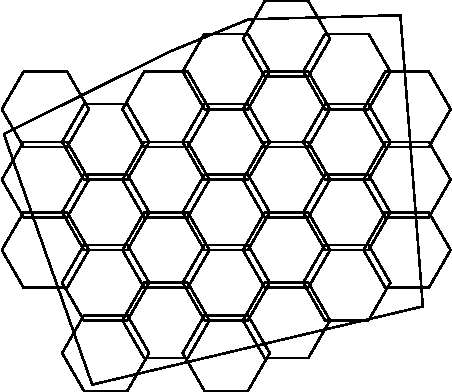
\includegraphics{README_files/figure-latex/unnamed-chunk-3-2.pdf}

\begin{Shaded}
\begin{Highlighting}[]
\CommentTok{\# st\_write(cuad\_final, \textquotesingle{}data/cuadricula{-}final.gpkg\textquotesingle{})}
\end{Highlighting}
\end{Shaded}

\hypertarget{referencias}{%
\section*{Referencias}\label{referencias}}
\addcontentsline{toc}{section}{Referencias}

\hypertarget{refs}{}
\begin{CSLReferences}{1}{0}
\leavevmode\hypertarget{ref-jose_ramon_martinez_batlle_2021_5694017}{}%
Batlle, J. R. M. (2021). {geofis/forest-loss-fire-reproducible: First
release} (Version v0.0.0.9000).
\url{https://doi.org/10.5281/zenodo.5694017}

\end{CSLReferences}

\end{document}
